% wave_temporal_corrected.tex
\documentclass[tikz,border=4pt]{standalone}
\usepackage{pgfplots}
\pgfplotsset{compat=1.18}
\renewcommand{\familydefault}{\sfdefault}

\begin{document}
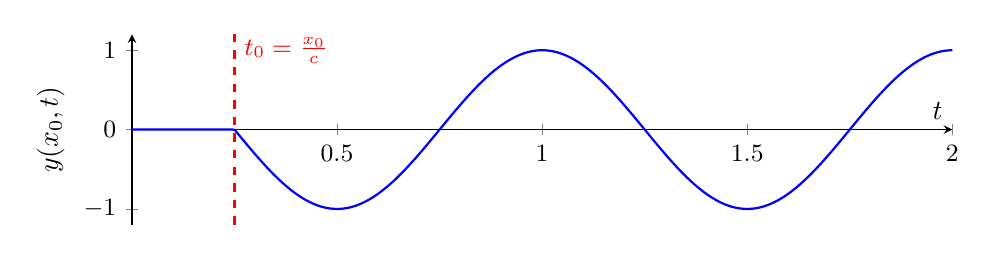
\begin{tikzpicture}
\pgfmathsetmacro{\A}{1}          % Amplitude
\pgfmathsetmacro{\lambda}{1}     % Wellenlänge
\pgfmathsetmacro{\c}{1}          % Ausbreitungsgeschwindigkeit
\pgfmathsetmacro{\k}{2*pi/\lambda}
\pgfmathsetmacro{\omega}{2*pi}   % Kreisfrequenz (f=1 Hz)
\pgfmathsetmacro{\xzero}{0.25}   % fester Ort x0
\pgfmathsetmacro{\tmax}{2}       % Zeitbereich (s)

% Verzögerung t0, bis Welle x0 erreicht
\pgfmathsetmacro{\tzero}{\xzero/\c}

\begin{axis}[
    width=12cm, height=4cm,
    xmin=0, xmax=\tmax,
    ymin=-1.2, ymax=1.2,
    axis x line=middle, axis y line=left,
    xlabel={$t$}, ylabel={$y(x_0,t)$},
    xtick={0,0.5,1,1.5,2},
    ytick={-1,0,1},
    ticklabel style={font=\small},
    every axis plot/.append style={thick, blue},
    clip=false
]

% Zeitliche Schwingung am Ort x0 (verschoben um t0)
\addplot[samples=400,domain=0:\tmax] 
    { (\x<\tzero) * 0 + (\x>=\tzero) * - \A * sin(deg(\omega*(\x-\tzero))) };

% Markierung wann die Welle x0 erreicht
\addplot[dashed,red] coordinates {(\tzero,-1.2) (\tzero,1.2)};
\node[anchor=west,font=\small, red] at (axis cs:\tzero,1) {$t_0 = \frac{x_0}{c}$};

\end{axis}
\end{tikzpicture}
\end{document}
